\documentclass[a5paper]{article}
\usepackage[a5paper, top=8mm, bottom=8mm, left=8mm, right=8mm]{geometry}

\usepackage{polyglossia}
\setdefaultlanguage[babelshorthands=true]{russian}

\usepackage{fontspec}
\setmainfont{FreeSerif}
\newfontfamily{\russianfonttt}[Scale=0.7]{DejaVuSansMono}

\usepackage[font=scriptsize]{caption}

\usepackage{amsmath}
\usepackage{amssymb,amsfonts,textcomp}
\usepackage{color}
\usepackage{array}
\usepackage{hhline}
\usepackage{cite}
\usepackage{ulem}

\usepackage[xetex,linktocpage=true,plainpages=false,pdfpagelabels=false]{hyperref}
\hypersetup{colorlinks=true, linkcolor=blue, citecolor=blue, filecolor=blue, urlcolor=blue, pdftitle=1, pdfauthor=, pdfsubject=, pdfkeywords=}

\usepackage{tabu}

\usepackage{graphicx}
\usepackage{indentfirst}
\usepackage{multirow}
\usepackage{subfig}
\usepackage{footnote}
\usepackage{listings}
\usepackage{minted}

\sloppy
\pagestyle{plain}

\title{Практика 1: Введение, потоки}

\date{16.02.2018г}

\begin{document}

\maketitle
\thispagestyle{empty}

\section{Формальности}
Итак, начинается вторая часть изучения программирования на примере языка Java. Пары в этом семестре будут логическим продолжением того, что было в предыдущем семестре --- немножко больше многопоточности, программирования сетевых приложений, многопоточных И сетевых приложений, приложений с пользовательским интерфейсом наконец-то, и даже немного веб-приложений, если мы до них дойдём. Как я понял, так или иначе почти всё затрагивалось при программировании под android, но в этот раз всё будет более системным и обстоятельным.

Сначала, как водится в начале семестра, формальности. В конце будет экзамен, оценка за который получается, в том числе, и из оценки по практике, так что в этом семестре будет не просто зачёт/незачёт, а некоторое число. Чтобы получить оную оценку, надо, как обычно, качественно и вовремя делать домашки, писать контрольные, сдавать их через HwProj (\url{http://hwproj.me/courses/26}), делая пуллреквест в свой репозиторий и кидая в HwProj ссылку на пуллреквест. В HwProj надо записаться на второй семестр этого курса. Домашек будет меньше, чем в прошлом семестре, но они будут более объёмными. Списывать, как обычно, нельзя, и вообще, имеет смысл стараться решать задачи самостоятельно, курс ориентирован на сольное прохождение, к тому же, если что --- всегда можно спросить у меня.

Пары у нас будут один раз в две недели, поэтому будет меньше времени практиковаться, но домашек особо меньше не будет. На самом деле, на парах я в основном буду что-то рассказывать.

Напомню про то, за что снимались баллы в прошлом семестре:\nopagebreak

\vspace{3mm}
\begin{small}
	\begin{tabu} {| X[1 l p] | X[0.3 l p] |}
		\tabucline-
		\everyrow{\tabucline-}
		Пропущенный дедлайн                                                                   & баллы делятся на два \\
		Задача на момент дедлайна не реализует все требования условия                         & пропорционально объёму невыполненных требований \\
		Неумение пользоваться гитом                                                           & -2 \\
		Проблемы со сборкой (в том числе, забытый org.jetbrains.annotations)                  & -2 \\
		Отсутствие JavaDoc-ов для всех классов, интерфейсов и паблик-методов                  & -2 \\
		Отсутствие описания метода в целом                                                    & -1 \\
		Слишком широкие области видимости для полей                                           & -2 \\
		if (...) return true; else return false;                                              & -2 \\
		Именование классов-полей-методов-... и прочие code convertions                        & -1 \\
		Неиспользование try-with-resources там, где это было бы уместно                       & -1 \\
		Комментарии для параметров с заглавной буквы                                          & -0.5 \\
	\end{tabu}
\end{small}
\vspace{3mm}

Обнаружение ошибок из этого списка сразу влечёт снятие баллов за задачу, даже без права исправить ошибку. На остальные ошибки я буду указывать и будет возможность их поправить, но наиболее распространённые ошибки будут пополнять этот список, так что имеет смысл ходить на пары, чтобы вовремя узнать, что меня в очередной раз ужаснуло и заставило расширить список ``плохих'' ошибок. Табличку с оценками я выложу на вики.

\section{Многопоточность}

Теперь перейдём к содержательной части пары. На теории вы уже должны были начать потоки, поэтому я ещё немного про них расскажу и немного попрактикуемся (а в домашке попрактикуетесь много).

Вообще многопоточные программы надо уметь писать, потмоу что нынче даже в телефонах процессоры имеют по четыре ядра, не говоря уже о настольных компьютерах и ноутбуках. Сильно грузить одно ядро, чтобы при этом остальные простаивали --- страшный грех нынче. Но дело не только в высокопроизводительных вычислениях (которые всё-таки не так часто встречаются) --- многопоточные программы позволяют пользователю продолжать взаимодействовать с интерфейсом и иметь возможность узнать прогресс длительной операции, или вообще её отменить. При этом длительная операция не обязательно длительная, потому что её считать сложно --- нет, это может быть, например, сетевой запрос, инициализация какого-нибудь устройства, да даже просто загрузка большого файла (или набора файлов, что часто приходится делать, например, в играх). Такие операции вообще не грузят процессор, поэтому, кстати, их можно запускать несколько сразу одновременно, чем пользуются, например, торрент-клиенты --- передаваемый файл разделяется на кучу маленьких кусков, каждый из которых качается независимо в отдельном потоке. Игры грузят много файлов тоже как правило в несколько потоков одновременно. Есть ещё чисто практическое соображение в пользу многопоточности --- на любом уважающем себя собеседовании про многопоточность будут вопросы.

Но иногда неопытные программисты, узнав о потоках, начинают вставлять их повсюду, что на самом деле приводит к разрушительным последствиям. Многопоточные программы гораздо сложнее в отладке, могут содержать сложнообнаружимые баги и вообще отличаются непредсказуемостью поведения. К тому же, не факт, что многопоточная программа будет работать быстрее такой же однопоточной --- переключение между потоками имеет свою цену с точки зрения производительности, а неграмотное использование потоков может заставить процессор тратить 95\% рабочего времени на обслуживание потоков. Так что много потоков --- не панацея, и надо такие программы писать очень аккуратно.

Немного про способы прострелить себе ногу: концептуально их всего два, состояние гонки (race condition) и взаимная блокировка потоков (deadlock).

\section{Состояние гонки}

Состояние гонки --- это любая ситуация, когда результат работы программы зависит от переключения потоков планировщиком. Эта ситуация во всех практических случаях считается ошибкой, потому что предсказать поведение планировщика нельзя и внешне всё выглядит так, будто результат работы программы случаен. Типичный пример гонки показан на картинке:

\begin{center}
	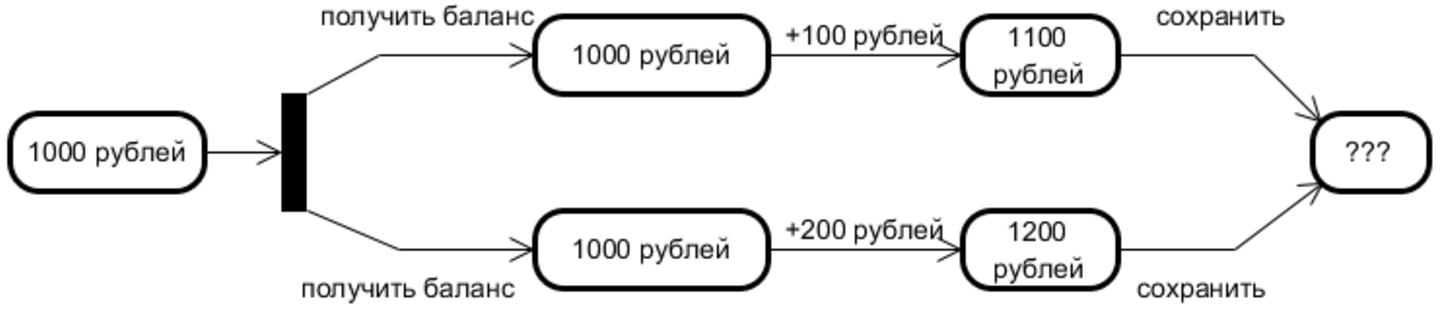
\includegraphics[width=\textwidth]{raceCondition.png}
\end{center}

Положим, что два потока одновременно хотят обновить баланс. Если планировщик сначала даст поработать первому потоку, тот считает значение текущего баланса, тут может так случиться, что планировщик остановит его и даст поработать второму потоку. Второй поток тоже считает текущее значчение баланса (то же, его ведь ещё не обновили), прибавит к нему 200 рублей и сохранит результат, в итоге обновлённый баланс будет 1200 рублей. Тут планировщик видит, что поток 2 завершён и даст доработать потоку 1, который прибавит 100 рублей к считанной им ранее сумме баланса, получив 1100 рублей, и радостно сохранит эти самые 1100 рублей в качестве текущего баланса. 200 рублей потеряно. А могло получиться и наоборот, и потерялись бы 100 рублей, что хотя и вдвое меньше, но тоже не очень.

Такая ситуация может быть слишком редкой, чтобы её надёжно воспроизвести, но в этом и проблема с гонками --- программа может работать правильно большую часть времени, примерно раз в 10 лет теряя одну транзакцию. Вот пример программы, которая, скорее всего, будет работать странно достаточно часто:

\begin{minted}{java}
int[] a = new int[1000];
for (int i = 0; i < a.length; ++i) {
    a[i] = 1;
}

int[] result = new int[1];

for (int i = 0; i < 100; ++i) {
    final int localI = i;
    new Thread(() -> {
        for (int j = localI * 10; j <= (localI + 1) * 10 - 1; ++j) {
            result[0] += a[j];
        }
    }).start();
}

Thread.sleep(100);

System.out.println("Result = " + result[0]);
\end{minted}

Берём массив из тысячи элементов, заполнняем его единицами, и хотим посчитать сумму чисел, которые в нём лежат, раз уж мы умные, в 100 потоков. Для этого делим массив на одинаковые куски по 10 элементов и суммируем каждый кусок в отдельном потоке, обновляя общую для всех потоков переменную с результатом. Обратите внимание на странные приёмы, которые тут используются --- переменная localI заведена, чтобы в замыкание в лямбда-функцию, которая будет работать в отдельном потоке, попало именно текущее значение i, а не счётчик цикла (иначе это ошибка компиляции), а массив из одного элемента --- это бюджетный способ получить мутабельное int-овое значение на куче. Так в продакшн-коде лучше не делать, но зато на слайд помещается. Ещё мы тут не пытаемся дождаться выполнения всех потоков, а просто надеемся, что они завершатся за 100 миллисекунд, так тоже в продакшн-коде делать нельзя (впрочем, тут, скорее всего, большинство потоков успеет завершиться до того, как стартуют следующие за ними, благо считать каждому потоку особо нечего). 

Этот пример можно запустить и посмотреть, что будет. Иногда получается 1000, иногда 999, а иногда и 992. Если мы сделаем более грамотно и сначала создадим все потоки, а потом всех их одновременно запустим, то по идее должно быть ещё хуже. Почему получается что-то странное? Операция ``+='' не атомарна, так что получается как на картинке --- один поток считал значение result[0], второй поток считал то же значение, прибавил, записал, первый поток тоже прибавил и тоже записал, затерев изменения второго.

Обратите внимание, что эта ситуация не специфична для Java, процессоров Intel или ещё чего-нибудь, так можно испортить себе программу где угодно. Бывают и более странные случаи гонок, о которых вам либо уже рассказали, либо расскажут на лекциях, связанные с перестановкой инструкций на конвейере процессора, наличием в процессоре write buffer-ов и т.д. А ещё компилятор имеет право менять порядок вычислений в целях оптимизации, и делает он это без учёта того, что другие потоки могут использовать промежуточные результаты этих вычислений.

\section{Deadlock}

Второй способ прострелить себе ногу --- когда поток ждёт наступления какого-нибудь события, которое наступит, только если поток продолжит работу, чего он сделать не может, поскольку ждёт наступления этого события. Например, когда двум потокам нужно два файла, чтобы работать, первый поток успел открыть первый файл, второй поток успел открыть второй, и оба ждут, пока другой нужный им файл освободится. При этом ни один поток не может продвинуться, поэтому не может и освободить файл:

\begin{center}
	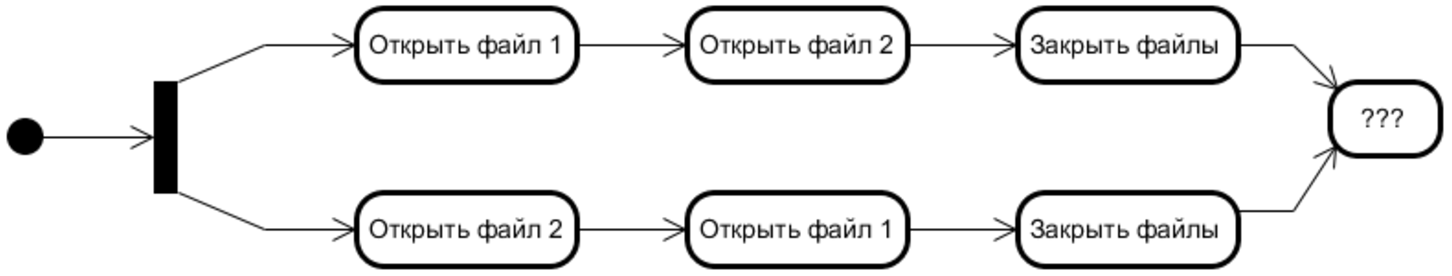
\includegraphics[width=\textwidth]{deadlock.png}
\end{center}

Самый простой способ добиться этой ситуации в программе --- это

\begin{minted}{java}
Thread.currentThread().join();
\end{minted}

--- поток ждёт, пока он же не завершится, но он не может завершиться, потому что он ждёт. Естественно, это игрушечный пример, но в реальной жизни заблокироваться на самом себе тоже совсем несложно --- например, неаккуратная работа с рекурсией (к счастью, встроенные в Java механизмы синхронизации с рекурсией работать умеют), хитрые схемы многопоточной обработки событий, когда один поток послал сигнал и ждёт на него ответа, чтобы получить который он должен ответить на какой-то другой сигнал.

Хорошая новость в том, что блокировка потока в принципе возможна только если выполняются одновременно четыре условия:
\begin{itemize}
	\item потокам нужен доступ к неразделяемому ресурсу, то есть ресурсу, владеть которым в каждый момент времени может только один поток;
	\item поток удерживает хотя бы один ресурс, ожидая доступа к другому ресурсу;
	\item у потока нельзя ``отнять'' ресурс, то есть он может освободить его только сам;
	\item каждый поток ожидает ресурса, занятого каким-то другим потоком, то есть имеется цикл зависимости по ресурсам.
\end{itemize}

Если хоть одно из этих условий не выполнено, то блокировка в принципе невозможна, поэтому проблему с блокировками можно решить, делая невозможным наступление одного из четырёх этих условий. Lock-free-подход --- ``нет неразделяемых ресурсов --- нет проблем'', подход, реализованный в C++-ном std::lock --- ``если лочить ресурсы всегда в одинаковом порядке, то не будет циклов'' и т.д. У нас же ресурсами будут, как правило, критические секции кода, они по определению неразделяемы, и надо внимательно следить, чтобы не пытаться синхронизироваться сразу по нескольким разделяемым переменным в неправильном порядке.

\section{Потоки в Windows}

Потоки в Java не обязаны отображаться напрямую в потоки операционной системы, но тем не менее в стандартной реализации отображаются. Так что понимать, что такое поток в операционной системе, было бы нелишне (хотя, конечно, это должны рассказывать на курсах про ОС, напомнить не помешает). Конкретно в Windows поток представляет собой некоторое количество записей в пространстве ядра и в пользовательском адресном пространстве, а именно:

\begin{itemize}
	\item Thread Kernel Object (\textasciitilde1240 байт)
	\item Thread environment block (TEB) (4 Кб)
	\item User-mode stack (1 Мб)
	\item Kernel-mode stack (24 Кб)
\end{itemize}

Потоку, как только он создаётся, сразу выделяется 1 мегабайт оперативки под стек, и поток может попросить у ОС увеличить размеры стека. Казалось бы, мелочь, но вспомните пример про сложение единиц в массиве, там мы создали 100 потоков, минус 100 мегабайт оперативной памяти сразу. Тоже, казалось бы, мелочь, но вот скриншот диспетчера задач моего ноутбука сразу после старта винды:

\begin{center}
	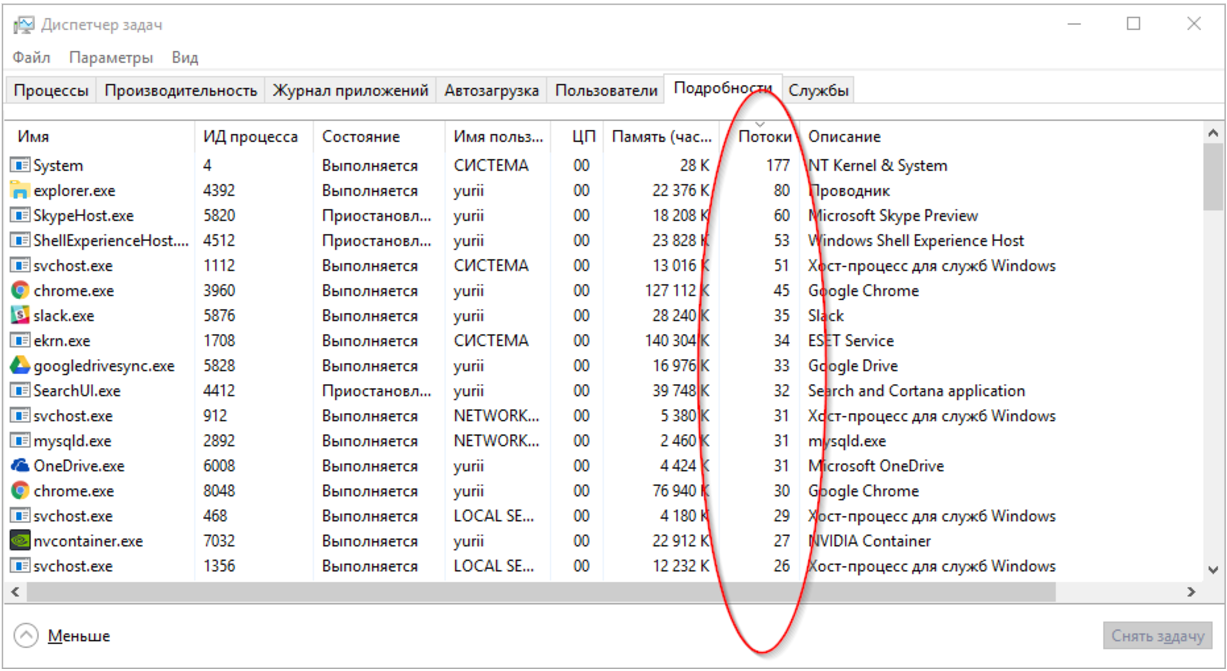
\includegraphics[width=0.85\textwidth]{threadsEverywhere.png}
\end{center}

Все эти потоки большую часть времени проводят в спящем режиме, так что процессорного времени не требуют, но оперативку под стек каждому потоку всё-таки надо. А их тысячи. Ещё, кстати, для каждой загруженной в приложение нативной разделяемой библиотеки (включая kernel32.dll, user32.dll, msvcrt32.dll и прочие подобные вещи) при запуске \textit{каждого} потока вызывается функция DllMain с параметрами DLL\_THREAD\_ATTACH и при завершении \textit{каждого} потока --- DLL\_THREAD\_DETACH. Библиотека вправе на эти параметры не реагировать (и большинство так и делают), но вызвана функция всё равно будет. Обычное нативное приложение грузит десятки разделяемых библиотек (свои, фреймворка, на котором оно написано, ядра Windows), так что это удар ещё и по производительности (к счастью, Java и .NET не используют эту чудо-систему). 

Поэтому желательно проектировать программу не как набор потоков, а как набор \textit{задач}, каждая из которых может выполняться в отдельном потоке, но отрабатывает быстро, поэтому потоки можно переиспользовать. Пулы потоков, которые реализованы в любой нормальной стандартной библиотеке современных языков, в том числе Java, как раз для поддержки такой парадигмы.

\section{Задача на дом}

Теперь про условие домашней задачи (на три недели, она относительно большая):
\begin{itemize}
	\item нужно реализовать класс ThreadPoolImpl, представляющий собой пул задач с фиксированным числом потоков (число задается в конструкторе);
	\item при создании объекта ThreadPoolImpl в нём должно начать работу n потоков;
	\item у каждого потока есть два состояния: ожидание задачи и выполнение задачи;
	\item задача --- вычисление некоторого значения, вызов get у объекта типа \textit{Supplier<R>};
	\item при добавлении задачи, если в пуле есть ожидающий поток, то он должен приступить к ее исполнению. Иначе задача будет ожидать исполнения, пока не освободится какой-нибудь поток;
	\item задачи, принятые к исполнению, представлены в виде объектов интерфейса LightFuture, про который подробнее дальше;
	\item у ThreadPoolImpl должен быть метод shutdown, который завершает работу всех потоков (через Thread.interrupt()).
\end{itemize}

LightFuture --- ссылка на значение, которое станет доступно когда-то в будущем. Это должен быть генерик (параметризованный типом возвращаемого значения), имеющий следующие методы:

\begin{itemize}
	\item isReady, который возвращает true, если задача выполнена;
	\item get, который возвращает результат выполнения задачи или блокирует вызывающего до тех пор, пока задача не будет выполнена;
	\begin{itemize}
		\item в случае, если соответствующий задаче supplier завершился с исключением, этот метод должен завершиться с исключением LightExecutionException;
	\end{itemize}
	\item thenApply --- принимает объект типа Function, который может быть применен к результату данной задачи X и возвращает новую задачу Y, принятую к исполнению. При этом:
	\begin{itemize}
		\item новая задача будет исполнена не ранее, чем завершится исходная;
		\item в качестве аргумента объекту Function будет передан результат исходной задачи, и все Y должны исполняться на общих основаниях (т.е. должны разделяться между потоками пула);
		\item метод thenApply может быть вызван несколько раз;
		\item метод thenApply не должен блокировать работу потока, если результат задачи X ещё не вычислен.
	\end{itemize}
\end{itemize}

Использование такого пула потоков может выглядеть, например, вот так:
\begin{minted}{java}
ThreadPoolmpl<Integer> pool = new ThreadPoolmpl<>(5);
LightFuture<Integer> task = pool.addTask(() -> 2 * 2);
assertThat(task.get(), is(4));

LightFuture<Integer> task1 = pool.addTask(() -> 2 * 3);
LightFuture<Integer> task2 = task1.thenApply((i) -> i + 1);
LightFuture<Integer> task3 = task1.thenApply((i) -> i + 2);
assertThat(task1.get(), is(6));
assertThat(task2.get(), is(7));
assertThat(task3.get(), is(8));
\end{minted}

Естественно, возможны варианты, напирмер, LightFuture можно сделать вложенным классом ThreadPoolImpl-а.

Кроме этого, ещё хочется следующего:
\begin{itemize}
	\item не использовать пакет java.util.concurrent, потому что там это уже реализовано, причём по-настоящему;
	\item все интерфейсные методы должны быть потокобезопасны, то есть и пул потоков, и LightFuture сами могут использоваться из нескольких потоков одновременно;
	\item для каждого базового сценария использования должен быть написан тест;
	\item обязателен билд в CI, на котором проходят ваши тесты;
	\item дедлайн: до \textbf{10:00 09.03.2018}.
\end{itemize}

\section{Задача на остаток пары}

Реализовать интерфейс, представляющий ленивое вычисление:

\begin{minted}{java}
public interface Lazy<T> {
  T get();
}
\end{minted}

Есть некоторое вычисление, представляемое объектом \textit{Supplier<T>}, его должно быть можно обернуть в реализацию \textit{Lazy<T>}, которая выполнит вычисление при первом обращении к методу \textit{get()}. При последующих обращениях к методу \textit{get()} должен возвращаться уже посчитанный результат, \textit{Supplier} второй раз вызываться не должен (вычисление вообще не должно производиться более одного раза). То есть отработавший \textit{Supplier} становится больше не нужен в \textit{Lazy} и его можно смело удалить.

Поскольку это задача на многопоточность, реализаций должно быть две:
\begin{itemize}
	\item однопоточная реализация, гарантирующая корректную работу, если поток всего один;
	\item многопоточная реализация, гарантирующая корректную, но несколько более медленную работу в случае, когда с \textit{Lazy} могут быть обращения из нескольких потоков сразу.
\end{itemize}

А поскольку у нас есть две реализации одного интерфейса, создавать их надо не вручную, а сделав класс \textit{LazyFactory}, у которого есть два статических метода вида \textit{public static <T> Lazy<T> create...Lazy(Supplier<T>)}, возвращающих либо первую реализацию, либо вторую.

При этом:
\begin{itemize}
	\item каждый объект \textit{Lazy} должен иметь не больше двух полей (обратите внимание, \textit{объект}, статические поля допустимы);
	\item \textit{Supplier.get} вправе вернуть \textit{null};
	\item должны быть тесты:
	\begin{itemize}
		\item однопоточные, на разные хорошие и плохие случаи;
		\item многопоточные, на наличие гонок.
	\end{itemize}
\end{itemize}

Эту задачу надо доделать дома и сдать тоже через HwProj (дедлайн такой же, как у предыдущей задачи, до \textbf{10:00 09.03.2018}).

\end{document}
